\section{Flæðirit og sauðakóði}Hér skal gera flæðirit og sauðakóða nýtið ykkur https://draw.io. Þegar þið hafið lokið að gera flæðiritið farið í export-image og vistið grafið í skyrsla/img meðnafni "flowhart". í Þessu skjali skuluð þið gera sauðakóða 
Ef þið lesið ykkur til um hvernig rita eigi sauðakóða þá setjið þið in tilvitnun  svona : \cite{hartman1989writing}

Sauðakóða dæmi:\\
loop forewer\{
  drive(until done)\\
  ArmUp(30)\\
  armDon(30)\\
  clawOpen()\\
  drive(until done)\\
\}
\begin{figure}[h]
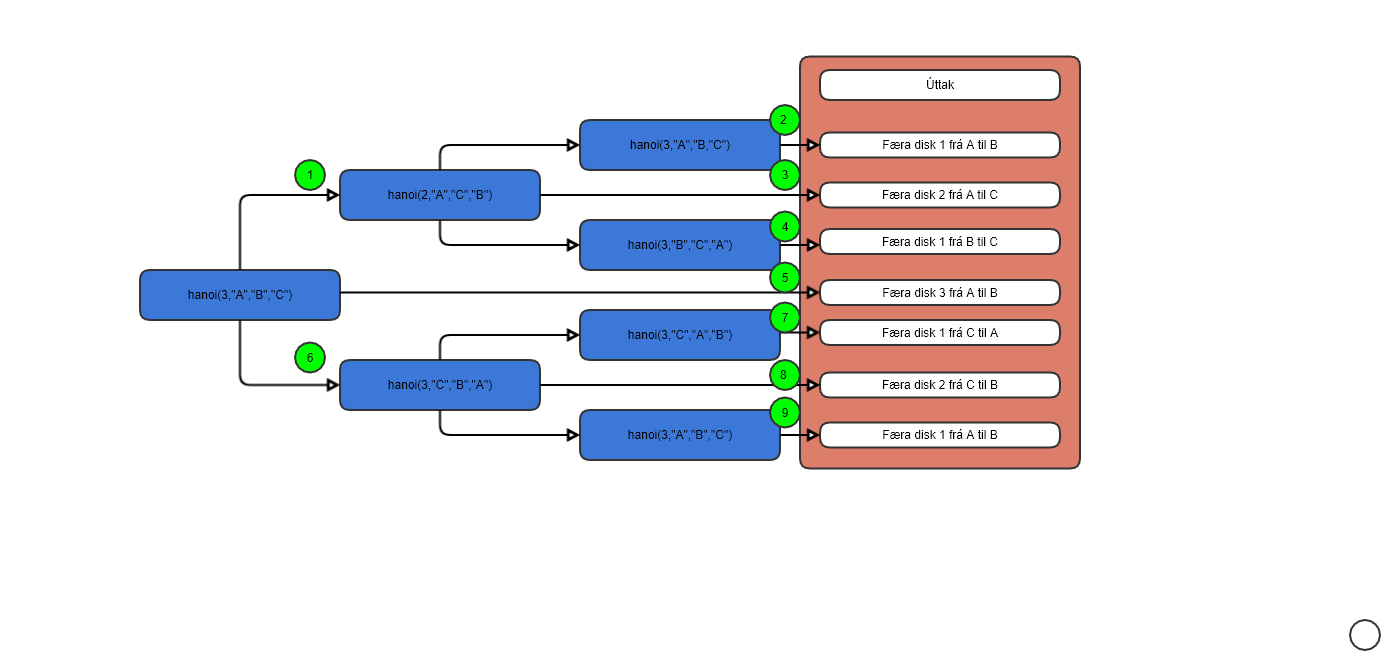
\includegraphics[scale=.3]{img/flowchart}
\end{figure}
